\documentclass[tikz,border=10pt]{standalone}
\usepackage{amsmath,amssymb}
\usetikzlibrary{calc,arrows.meta}

\begin{document}
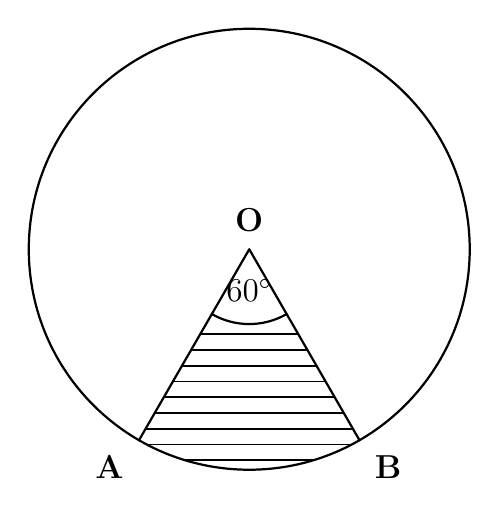
\begin{tikzpicture}[>=latex, line cap=round, line join=round]
  \def\R{2.8}

  % Coordinates
  \coordinate (O) at (0,0);
  \coordinate (A) at (-120:\R);
  \coordinate (B) at (-60:\R);

  % Shading / horizontal hatching inside sector AOB strictly BELOW the angle arc
  \begin{scope}
    \clip (O) -- (A) arc (-120:-60:\R) -- cycle;
    \foreach \y in {-1.08,-1.28,...,-2.8} {
      \draw[semithick] (-\R-0.2, \y) -- (\R+0.2, \y);
    }
  \end{scope}

  % Sector boundary lines
  \draw[thick] (O) -- (A);
  \draw[thick] (O) -- (B);

  % Circle outline
  \draw[thick] (O) circle (\R);

  % Central angle arc and label
  \draw[thick] (-120:0.95) arc (-120:-60:0.95);
  \node at (-90:0.52) {\large $60^\circ$};

  % Center node O
  \node[above=3pt] at (O) {\large $\mathbf{O}$};

  % Sector points A and B
  \node[below left=2pt] at (A) {\large $\mathbf{A}$};
  \node[below right=2pt] at (B) {\large $\mathbf{B}$};

\end{tikzpicture}
\end{document}
